\chapter{Method}
The method chapter gives a high level overview of the method used in this paper. More detailed steps are delegated to the results Chapter \ref{cha:Results}. Chapter \ref{cha:Results} contains implementation details and the evaluation of the implementation.

The problem is clearly defined from the previous chapters, especially Section \ref{sec:TheProblem} which goes into detail with examples. Alternatives for this implementation are then explored and presented to the project manager of the Spade compiler -- which also happens to be an author in this paper -- for evaluation and consideration, the motivation for picking these are discussed in Section \ref{sec:ImplementationAlt}. This allows a flexible approach to implementation where the goal is to find the simplest implementation. This way of working is a take on the agile methodologies.

After a viable solution is picked, it is time to implement that solution. Since the project is open source special care should be taken to make the changes easily accessible and available after this paper is written, since it is very much possible. A list of the repositories and versions of each software are available in the Appendix \ref{app:VersionsAndGitHashes} and the \href{https://github.com/FredTheDino/thesis-spade-lang}{git-repository for this thesis}. Steps of the implementation and details relevant to the results are discussed in the implementation details section -- Section \ref{sec:ImplementationDetails}. A full evaluation for each of the potential implementations and details about these implementations that are deemed relevant and interesting are mentioned. For full details it is probably best to read the source code. 

The implementation is then evaluated based on 7 example programs in Chapter \ref{cha:ImplementationEval} -- these programs are available in the Appendix \ref{app:Programs} and the \href{https://github.com/FredTheDino/thesis-spade-lang}{git-repository for this thesis}. The programs will also be evaluated by a place and route, this thesis uses nextpnr version \verb+0.6-29-g54b20457+ for all the PNR done in this thesis. All the statistics from the PNR step is then saved, and all the experiments are run at least fifty (50) times to give some credibility to the results. The most interesting metric is the number of LUTs used in the final design. The number of LUTs will be the primary basis of analysis.

This information is then presented in Chapter \ref{cha:Results} and discussed in Chapter \ref{cha:Discussion}.

\section{Finding Implementations and Creative Problem Solving}
Solving complex problems is a creative process. Programmings languages are required to be complex since the ideas expressed in them are themselves complex. Complex problems require complex tools. The complexity requires that the programming language
has a certain degree of quality -- else the programming language quickly becomes useless and frustrating to use. To find a solution of sufficient quality requires trial and error and a good dose of analysis. Understanding partial solutions to a complex problem is a natural way of finding a solution that is higher in quality and hopefully good enough for the programming language to be usable. The Figure \ref{figCreativeProcess} contains a visualization of how these steps integrate with each other.

\begin{center}
\begin{figure}[h!]
\centering
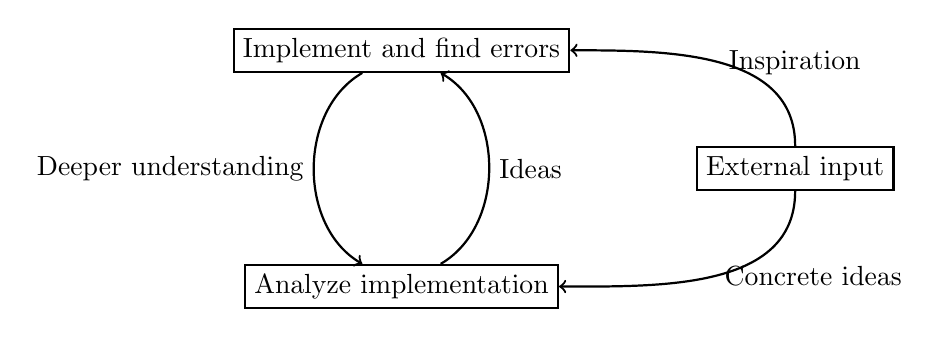
\begin{tikzpicture}[thick, node/.style = {draw}]
  \node[node] (a) at (0,0) {Analyze implementation};
  \node[node] (b) at (0,3) {Implement and find errors};
  \node[node] (c) at (5,1.5) {External input};

  \draw[->, align=left] (a) to[out=30,in=-30] node[right]{Ideas} (b);
  \draw[->, align=left] (b) to[out=-150,in=150] node[left]{Deeper understanding} (a);
  \draw[->] (c) to[out=-90,in=0] node[right]{Concrete ideas} (a);
  \draw[->] (c) to[out=90,in=0] node[right]{Inspiration} (b);
\end{tikzpicture}
\caption{The creative process of solving complex problems according to the author.}
\label{figCreativeProcess}
\end{figure}
\end{center}

\Todo{Show the generics with ranges that can now be used}
